\chapter{Methods}
\label{chap:methods}

For the thesis format for BSU, here is an example Chapter.

\section{Summary}
 
This is an example of a Chapter. 

\section{Computaional Methods}

At the core of Morphct is the estimation of HOMO (for donor) and LUMO (acceptor). This is because 
the inputs into the marcus hopping equation are the offsets between neigboring  chromophores energy levels
determine the driving force and the the TI is estimated using a dimer method that also uses the homo level. 
With that said, quantum chemical methods give us a framework from whcih to estimate the homo/lumos. A litany of
methods that use approximations and parametrizations to transform cumbersome ab initio quantum mechanical 
calculations into efficient algorithms for determining the electronic stucuture of a given compound. Morpcht 
leverages MINDO/3, a variation of the INDO(Intermediate Neglect of Differential Overlap) method,
which is an approximation method that seeks recreate the ab initio Hartree-Fock results\cite{Thiel2014}. Results
from the this work compare well to jones2017 which implemented ZINDO/s, another semi-emperical method. A particular 
choice of method comes down to how well we can organize a workflow. 

\indent The software chosen to implement this method is
provided by pySCF (Python-based Simulations of Chemistry Framework) \cite{Sun2018a}. This framework
was chosen in the interest of reproducabilty and extensibilty. PySCF is implemented almost entirly in the Python 
language, which is becoming increasingly ubiquitious in the scientific computing community.
Solving shrodingers equation accross tens of thousands of 
chromophores, which will be required to model an OPV material on the order of 10 nm, is untenable. Therefore
justified but drastic simplifications are necessary. 

\section{\nobreak kmc analysis}
Taking a charge to be a quasi-particle inserted into a MD generated morpholgy, a KMC
simulation can be run on the bases of Marcus rates obtained from QCC.
The KMC algorithm allows an explicit calculation of the MSD accross a large number of 
particles in the system. Repeating along relevant time scales for 
charge transfer, knowing that MSD scales linearly with time, the slope of this relationship
can be estimated and related to to the 3D diffusion coeffiecient. Using the Einstien relation, 
the gorundwork for which Einstein derived in his doctoral dissertaion, finally the zero-field
mobility can be obtained. 

\begin{figure}
  \center
  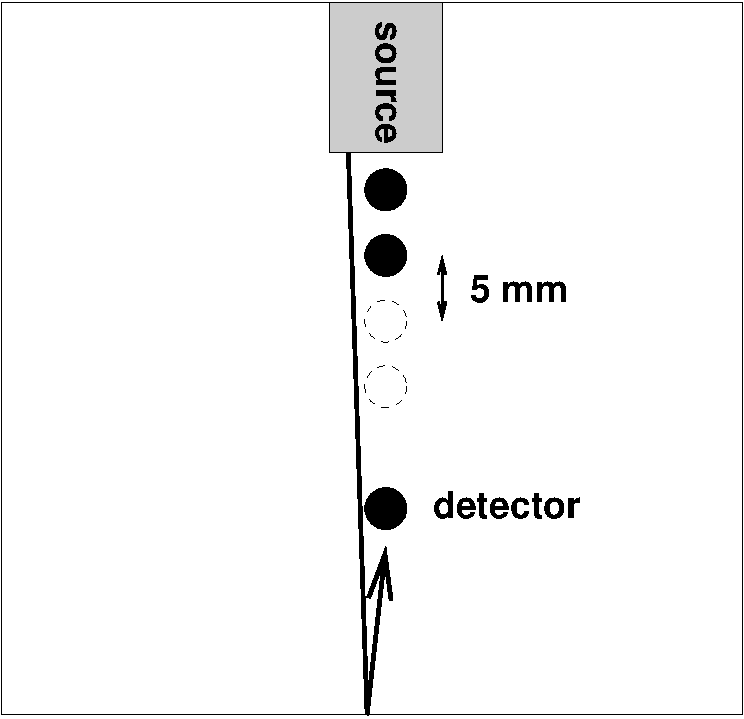
\includegraphics[width=7.5cm]{figures/setup}
  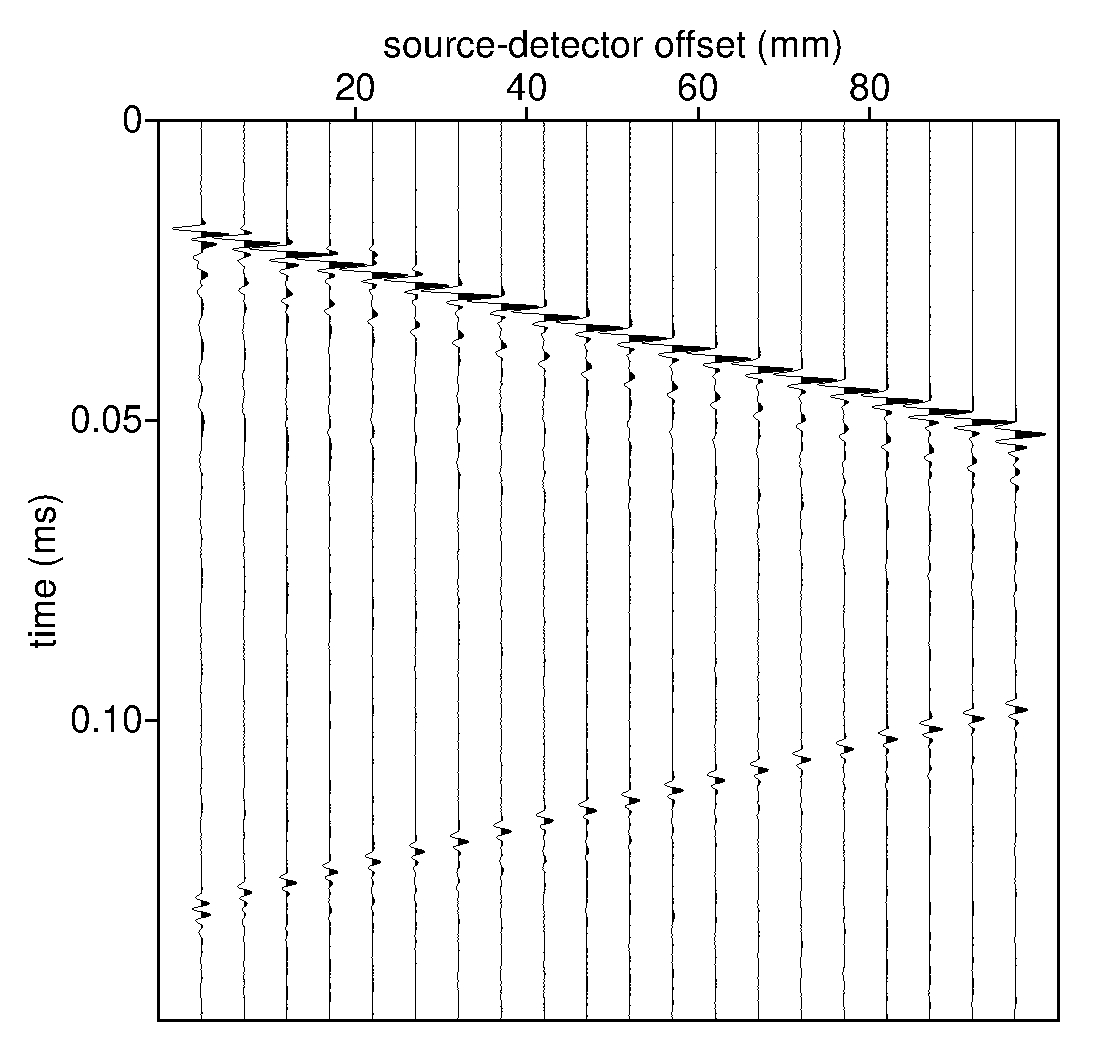
\includegraphics[width=7.5cm]{figures/exp0}
  \caption{Top-view of the experimental configuration (left) on the
    smooth face of aluminum.}
  \label{fig:figure}
\end{figure}

\subsection{Example of a subsection}

There are headings for chapters, sections, subsections and even
subsubsections:

\subsubsection{Appendices}

In Appendix~\ref{app:example} there is an example of an equation,
while 95\% confidence intervals for $\sigma$ are given in
Table~\ref{table:sigma}.
\begin{table}
  \caption{Approximate 95\% confidence intervals (in ms) for the true 
    standard deviation $\sigma=2.0$~ms of the VSP data. 
    The first column corresponds to the model-independent estimate, 
    the others are model-based estimates from the three different L-curves.} 
  \begin{center} 
    \begin{tabular}{|c|c|c|c|}\hline 
      $\sigma_\mu$  & $\sigma_I$ &$\sigma_{L}$  &$\sigma_{1/\lambda}$  \\
      \hline  
      2.02 $\pm$ 0.03 & 1.90 $\pm$ 0.03  & 1.92 $\pm$ 0.03 & 1.93 $\pm$ 0.03 
      \\ \hline 
    \end{tabular} 
    \label{table:sigma} 
  \end{center} 
\end{table} 

% usually, you'd let latex decide on the page breaks, but to create
% some pages for this template:
\newpage

more bla $\theta$ di bla (to create some more pages)

\begin{equation}
    M = \theta ^2
\end{equation}

\todo{Put something here!}
%\textcolor{red}{Put something here!}

\subsection{Abbreviations}

\gls{ny}, \gls{la} and \gls{un} are abbreviations whereas
% \gls{angelsperarea}, \gls{numofangels} and \gls{areaofneedle} are part of the nomenclature
First use: \gls{svm}. Second use: \gls{svm}.



\newpage 

and a little more...


%%% Local Variables: 
%%% mode: latex
%%% TeX-master: "BSUmain"
%%% End: 
